\documentclass[conference,final]{IEEEtran}

\usepackage{cite}
\usepackage[final]{graphicx}
\setkeys{Gin}{draft=false}
\usepackage{booktabs}
\usepackage{array}
\usepackage{url}
\usepackage{amsmath}
\graphicspath{{./figures/}{./docs/figures/}{./CampusFlow/docs/figures/}{./CampusFlow/CampusFlow/docs/figures/}}

\title{CampusFlow: A Unified Digital Placement Management System for Universities}

\author{
\begin{tabular}{ccc}
\multicolumn{3}{c}{\begin{minipage}[t]{0.70\textwidth}\centering
Mrs. S. Shanmugapriya\\[-1pt]
Department of Computer Science and Engineering\\
Kalasalingam Academy of Research and Education\\
Krishnankoil, India\\
somya87sankar@gmail.com
\end{minipage}} \\[1.2ex]
\begin{minipage}[t]{0.30\textwidth}\centering
G. Ajay\\[-1pt]
CSE (AI \& ML)\\
Kalasalingam Academy of Research and Education\\
Krishnankoil, India\\
reddyajay510@gmail.com
\end{minipage} &
\begin{minipage}[t]{0.30\textwidth}\centering
P. Venkata Sai Karthik\\[-1pt]
CSE (AI \& ML)\\
Kalasalingam Academy of Research and Education\\
Krishnankoil, India\\
pylasai43@gmail.com
\end{minipage} &
\begin{minipage}[t]{0.30\textwidth}\centering
G. Satya Sai\\[-1pt]
CSE (AI \& ML)\\
Kalasalingam Academy of Research and Education\\
Krishnankoil, India\\
satyasaigubbala640@gmail.com
\end{minipage} \\[1.2ex]
\begin{minipage}[t]{0.30\textwidth}\centering
Shaik Gayas Ali\\[-1pt]
CSE (AI \& ML)\\
Kalasalingam Academy of Research and Education\\
Krishnankoil, India\\
shaikgayasali@gmail.com
\end{minipage} & &
\\
\end{tabular}
}

\begin{document}

\maketitle

\begin{abstract}
We present CampusFlow, a web-based system for managing university placement drives and student applications. The platform brings together student profiles, company and drive records, rule-based eligibility checks, registration, shortlisting, recruitment stages, notifications, and placement analytics. Its browser client uses React and TypeScript; the backend is implemented with FastAPI and PostgreSQL. Eligibility rules are evaluated deterministically and return reasons for unmet criteria. We describe the system architecture, data flow, and drive lifecycle, then examine the functional scenarios represented in the repository's integration tests. These scenarios use synthetic records and cover a cross-role placement workflow and selected authorization boundaries. They do not establish production performance, user satisfaction, or placement outcomes. The paper therefore reports system design and software validation, not a field trial.
\end{abstract}

\begin{IEEEkeywords}
Campus placement, placement management system, eligibility evaluation, workflow automation, student information system, recruitment analytics.
\end{IEEEkeywords}

\section{Introduction}
University placement offices coordinate student records, employer requirements, application windows, shortlisting, interviews, and final outcomes. In many institutions these tasks are distributed across forms, spreadsheets, email, and messaging tools. Each tool may serve a local purpose, but staff then need to reconcile duplicate or outdated information and students may not know whether they satisfy a drive's criteria or what action is due next. Prior systems have also described web-based automation of placement-office processes and candidate searching [1].

CampusFlow treats placement as a sequence of linked records and state changes rather than as a collection of separate announcements. A placement officer creates a company-linked drive and configures eligibility criteria. A student views published opportunities, receives an eligibility result with reasons, and registers while the drive is open. Officers then manage applicants through ordered stages and publish outcomes. The same application provides role-specific views and administrative reporting.

This paper documents the implemented system and its verification scope. It does not claim that workflow automation alone improves placement rates, nor does it present a production load test. Its contributions are:
\begin{itemize}
    \item A lifecycle model linking drive publication, eligibility checks, student registration, stages, and results.
    \item A deterministic eligibility service that reports each failed criterion rather than producing an opaque ranking.
    \item A role-protected API and asynchronous notification path for placement events.
    \item A repository-grounded account of functional tests, their synthetic data, and the evaluation questions still open.
\end{itemize}

\section{Related Work}
Rathod and Shah describe an online system for student records and placement-office candidate searches [1]. Other reports cover internship profiles and eligibility [2], placement-office coordination [3], and student placement records with analytics [4]. CampusFlow shares their goal of consolidating placement tasks, while its implementation explicitly models drive transitions, ordered stages, explainable eligibility rules, and per-recipient notification tasks. This is a feature comparison, not a claim of superior effectiveness.

Role-based access control assigns permissions to organizational roles [5], a model used by CampusFlow's student, officer, and administrator API operations. Authentication uses JSON Web Tokens [6]; authorization is still enforced server-side for each resource.

Table~\ref{tab:comparison} compares the scope reported by the cited placement system with the features implemented in CampusFlow. ``NR'' means the feature was not reported in the cited description; it must not be interpreted as proof that the original system lacks it.

\begin{table*}[!t]
\caption{Feature Scope in the Cited System Description and CampusFlow}
\label{tab:comparison}
\centering
\small
\setlength{\tabcolsep}{3pt}
\begin{tabular}{p{0.14\textwidth}p{0.11\textwidth}p{0.14\textwidth}p{0.15\textwidth}p{0.15\textwidth}p{0.18\textwidth}}
\toprule
\textbf{System} & \textbf{Student records} & \textbf{Eligibility rules} & \textbf{Drive stages} & \textbf{Role-based API} & \textbf{Notifications / analytics} \\
\midrule
Rathod and Shah [1] & Reported & Candidate search reported & NR & Login reported; policy NR & NR \\
CampusFlow & Profile and academic records & Configurable deterministic rules & Ordered lifecycle and stage assignments & Student, officer, and admin guards & Async notification service and analytics endpoints \\
\bottomrule
\end{tabular}
\end{table*}

\section{System Architecture and Methodology}
CampusFlow follows a modular-monolith architecture. The browser client sends authenticated requests to the FastAPI application. API handlers validate input and enforce role checks, service classes apply workflow rules, repositories perform database operations, and PostgreSQL stores persistent records. Notification dispatch is separated from delivery: the application creates a task for a recipient, and a worker processes it asynchronously. Figure~\ref{fig:architecture} summarizes the runtime responsibilities represented in the code and deployment design.

\begin{figure*}[!t]
\centering
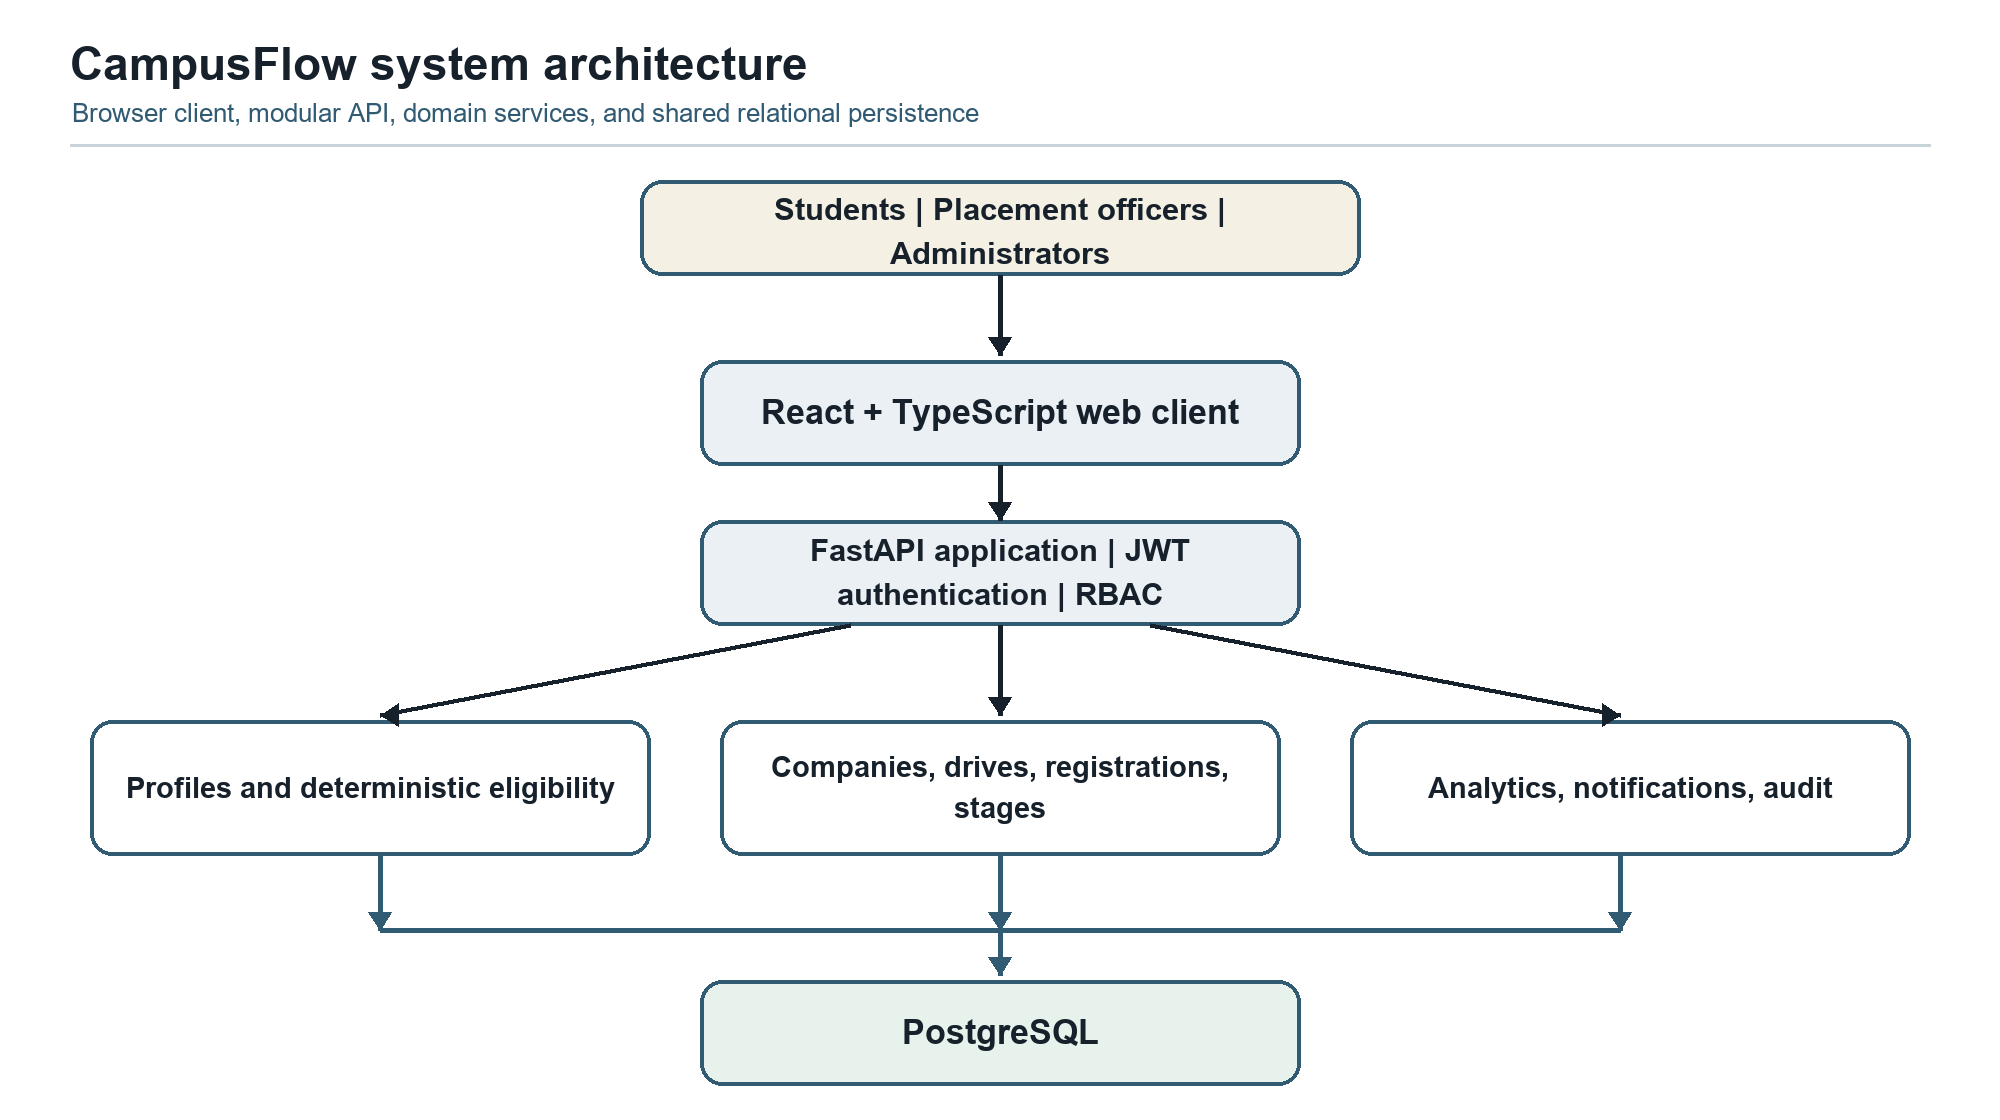
\includegraphics[width=0.84\textwidth]{campusflow_architecture.png}
\caption{CampusFlow's browser, API, domain-service, and persistence layers.}
\label{fig:architecture}
\end{figure*}

\begin{figure}[!t]
\centering
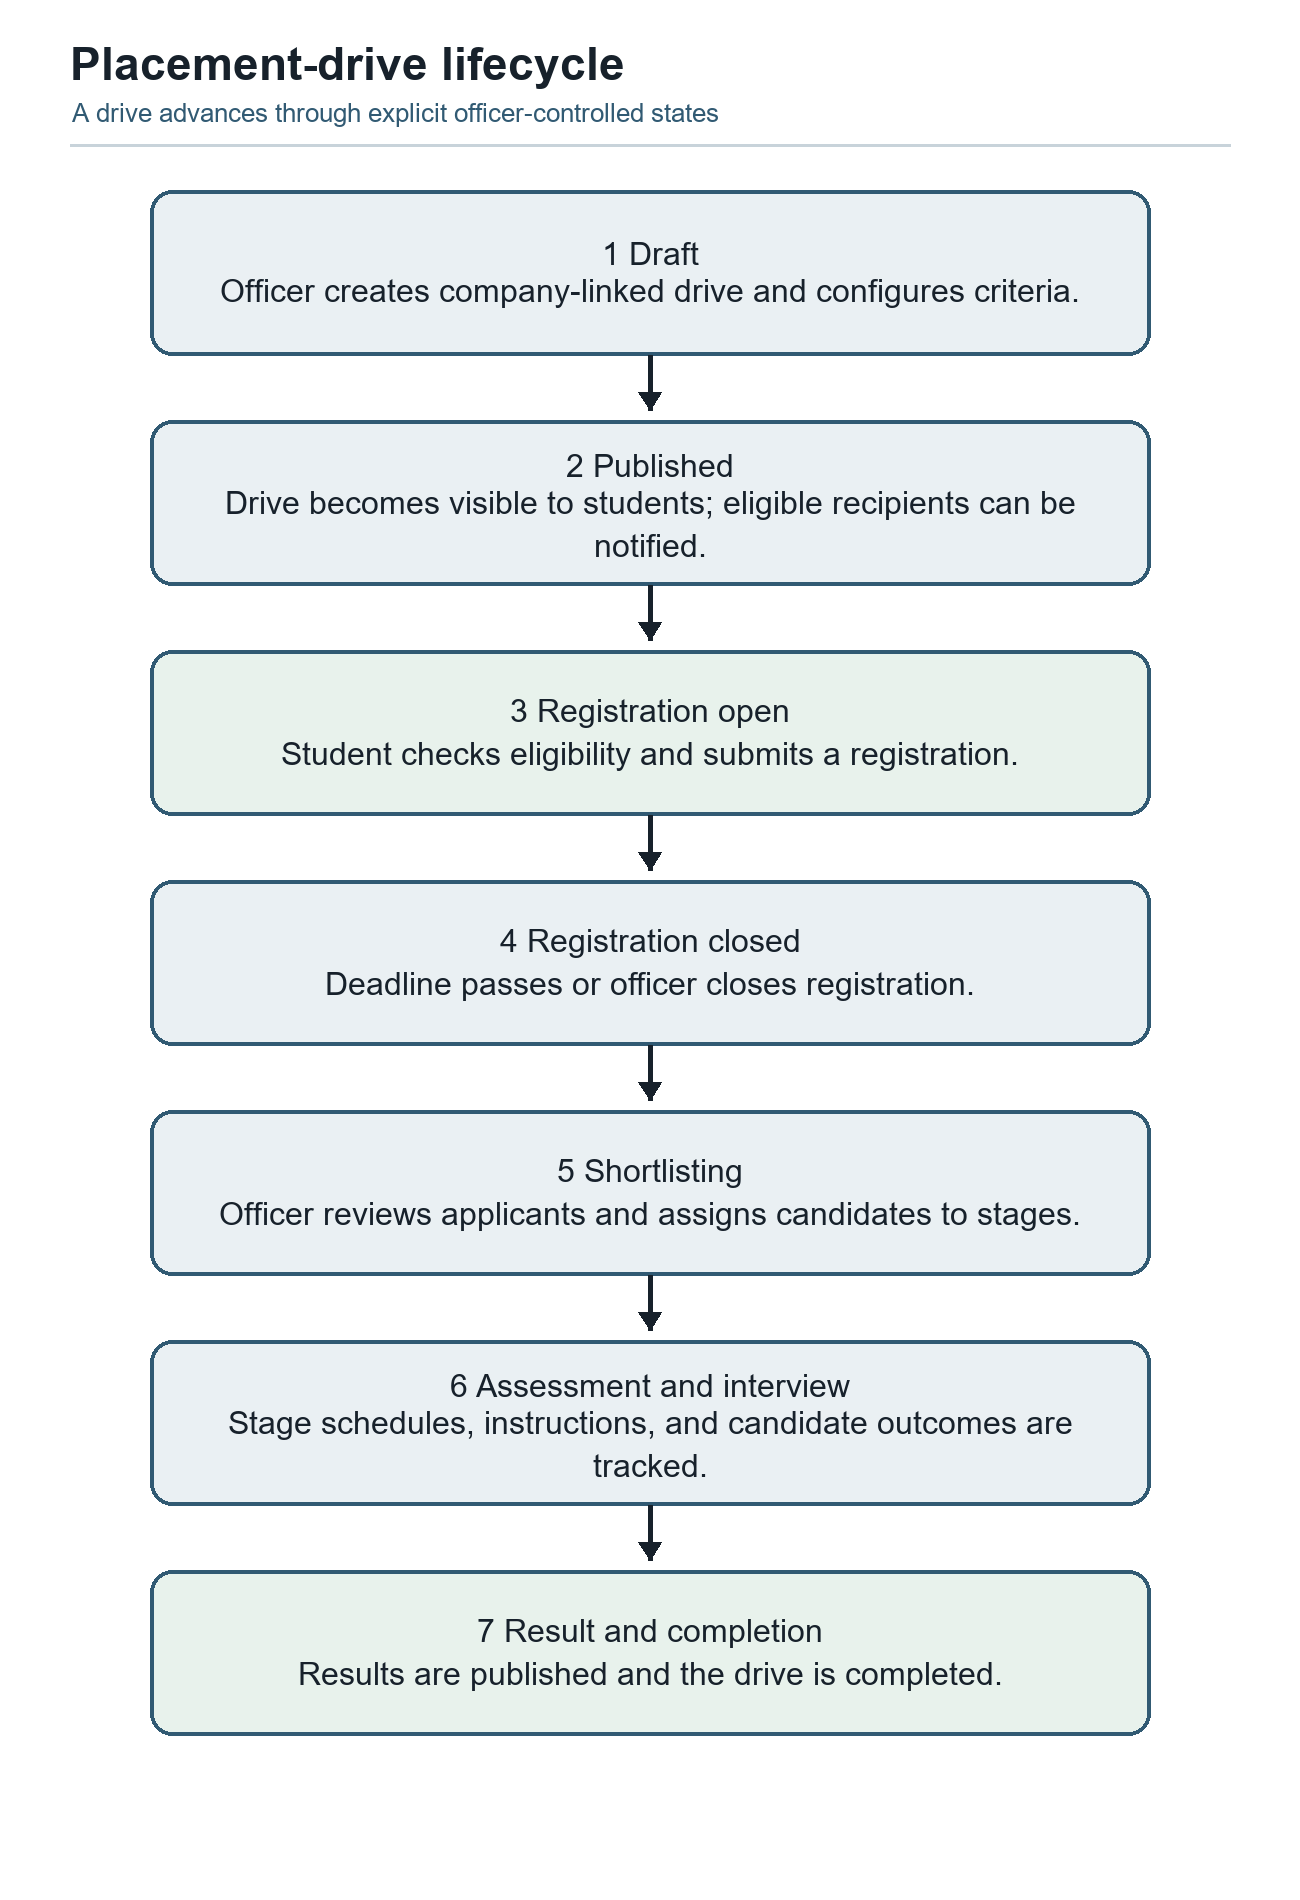
\includegraphics[width=0.76\columnwidth,height=0.64\textheight,keepaspectratio]{placement_lifecycle.png}
\caption{Placement-drive lifecycle implemented in CampusFlow.}
\label{fig:workflow}
\end{figure}

\subsection{Core Modules}
The primary modules and their responsibilities are summarized in Table~\ref{tab:modules}.

\begin{table}[t]
\caption{Core Modules and Responsibilities}
\label{tab:modules}
\centering
\small
\begin{tabular}{p{0.27\columnwidth} p{0.63\columnwidth}}
\toprule
\textbf{Module} & \textbf{Responsibility} \\
\midrule
Student profiles & Maintains academic, personal, and placement-related information. \\
Company and drives & Stores company details, job roles, drive information, and criteria. \\
Eligibility engine & Evaluates student profiles against drive-specific rules and returns reasons. \\
Registration and stages & Tracks registrations, shortlisting, interview stages, and outcomes. \\
Notifications & Delivers updates through configured notification channels. \\
Analytics & Summarizes registrations, placement stages, and outcomes. \\
Administration & Supports account, role, and system oversight. \\
\bottomrule
\end{tabular}
\end{table}

\subsection{Data Organization and Roles}
The relational model separates accounts from student-specific academic records and stores eligibility criteria independently from drive metadata. Registrations associate a student with a drive; stage assignments record progression within that drive. This separation allows one student profile to be evaluated against multiple drives without copying the profile into every application record.

Table~\ref{tab:entities} identifies the principal records used by the placement workflow. It is a conceptual view of the application model, not a complete database schema.

\begin{table}[!t]
\caption{Principal Placement Data Records}
\label{tab:entities}
\centering
\footnotesize
\begin{tabular}{p{0.29\columnwidth} p{0.59\columnwidth}}
\toprule
\textbf{Record} & \textbf{Purpose in the workflow} \\
\midrule
User & Stores identity, authentication state, and role. \\
Student profile & Stores roll number, branch, batch, CGPA, backlog count, and student attributes. \\
Company & Provides the organization linked to one or more placement drives. \\
Eligibility criteria & Stores per-drive rules evaluated against a student profile. \\
Registration & Records a student's application to a drive. \\
Stage and assignment & Stores ordered recruitment stages and student-level outcomes. \\
Notification and audit log & Records user-facing events and traceable administrative actions. \\
\bottomrule
\end{tabular}
\end{table}

Access depends on both role and resource ownership. Table~\ref{tab:permissions} summarizes the main responsibilities; enforcement is performed by backend routes and services, not by hiding frontend controls.

\begin{table}[!t]
\caption{Role Responsibilities}
\label{tab:permissions}
\centering
\footnotesize
\begin{tabular}{p{0.18\columnwidth} p{0.70\columnwidth}}
\toprule
\textbf{Role} & \textbf{Representative authorized operations} \\
\midrule
Student & Read and update permitted profile fields, view published drives, check own eligibility, register, and read own notifications. \\
Officer & Manage companies and drives, view applicants, define stages, shortlist students, publish results, and access placement analytics. \\
Administrator & Manage users and roles, inspect audit records, and perform administrative oversight. \\
\bottomrule
\end{tabular}
\end{table}

\subsection{Placement Workflow}
The workflow begins when a student maintains a profile containing academic and other placement-related information. A placement officer creates a company profile and a drive, defines its eligibility criteria, and publishes it to students. Students can review the drive, check their eligibility, and register when registration is open. Officers then manage shortlisting and subsequent assessment or interview stages. Results and placement status are recorded centrally, allowing authorized users to monitor progress.

The system enforces forward transitions through the drive lifecycle: draft, published, registration open, registration closed, shortlisting, assessment, interview, result, and completed. Figure~\ref{fig:workflow} summarizes the user-facing sequence. Table~\ref{tab:lifecycle} lists the transition order and the primary action.

\begin{table}[!t]
\caption{Placement-Drive State Progression}
\label{tab:lifecycle}
\centering
\footnotesize
\begin{tabular}{p{0.26\columnwidth} p{0.22\columnwidth} p{0.32\columnwidth}}
\toprule
\textbf{Current state} & \textbf{Next state} & \textbf{Primary action} \\
\midrule
Draft & Published & Officer publishes drive \\
Published & Reg. open & Officer opens registration \\
Reg. open & Reg. closed & Deadline or officer action \\
Reg. closed & Shortlisting & Officer begins review \\
Shortlisting & Assessment & First stage begins \\
Assessment & Interview & Assessment completes \\
Interview & Result & Officer publishes outcome \\
Result & Completed & Officer completes drive \\
\bottomrule
\end{tabular}
\end{table}

\subsection{Eligibility Evaluation}
Eligibility is determined using configurable rules rather than a learned prediction model. Criteria include minimum CGPA, maximum active backlogs, eligible branches, eligible batch years, and an optional gender criterion. For a profile $s$ and drive $d$, let $R(s,d)$ be the set of reasons returned by the configured checks. The implemented decision is:
\begin{equation}
    \operatorname{eligible}(s,d) = \begin{cases}
        1, & R(s,d)=\emptyset,\\
        0, & R(s,d)\ne\emptyset.
    \end{cases}
\end{equation}
All failed checks are accumulated so the response can explain more than one reason at once. Branch and gender comparisons are case-insensitive. The check is deterministic: the same profile and criteria produce the same result.

Table~\ref{tab:criteria} summarizes the criteria supported by the eligibility service.

\begin{table}[!t]
\caption{Eligibility Criteria Supported by the Engine}
\label{tab:criteria}
\centering
\footnotesize
\begin{tabular}{|p{0.16\columnwidth}|p{0.21\columnwidth}|p{0.43\columnwidth}|}
\hline
\textbf{Criterion} & \textbf{Example} & \textbf{Evaluation} \\
\hline
Minimum CGPA & 7.5 & Student CGPA must be at least 7.5. \\
\hline
Active backlogs & 0 allowed & Student backlog count must not exceed the configured limit. \\
\hline
Branch & CSE & Student branch must be in the configured list. \\
\hline
Batch year & 2026 & Student batch year must be in the configured list. \\
\hline
Gender (optional) & FEMALE & If configured, profile value must match without case sensitivity. \\
\hline
\end{tabular}
\end{table}

The integration test supplies a synthetic example: a CSE student in batch 2026 has CGPA 8.5 and no active backlogs; the drive permits CSE students in batch 2026 with CGPA of at least 7.5 and no backlogs. The expected decision is eligible. This documents a test fixture, not a real student record or population-level accuracy result.

\begin{figure*}[!t]
\centering
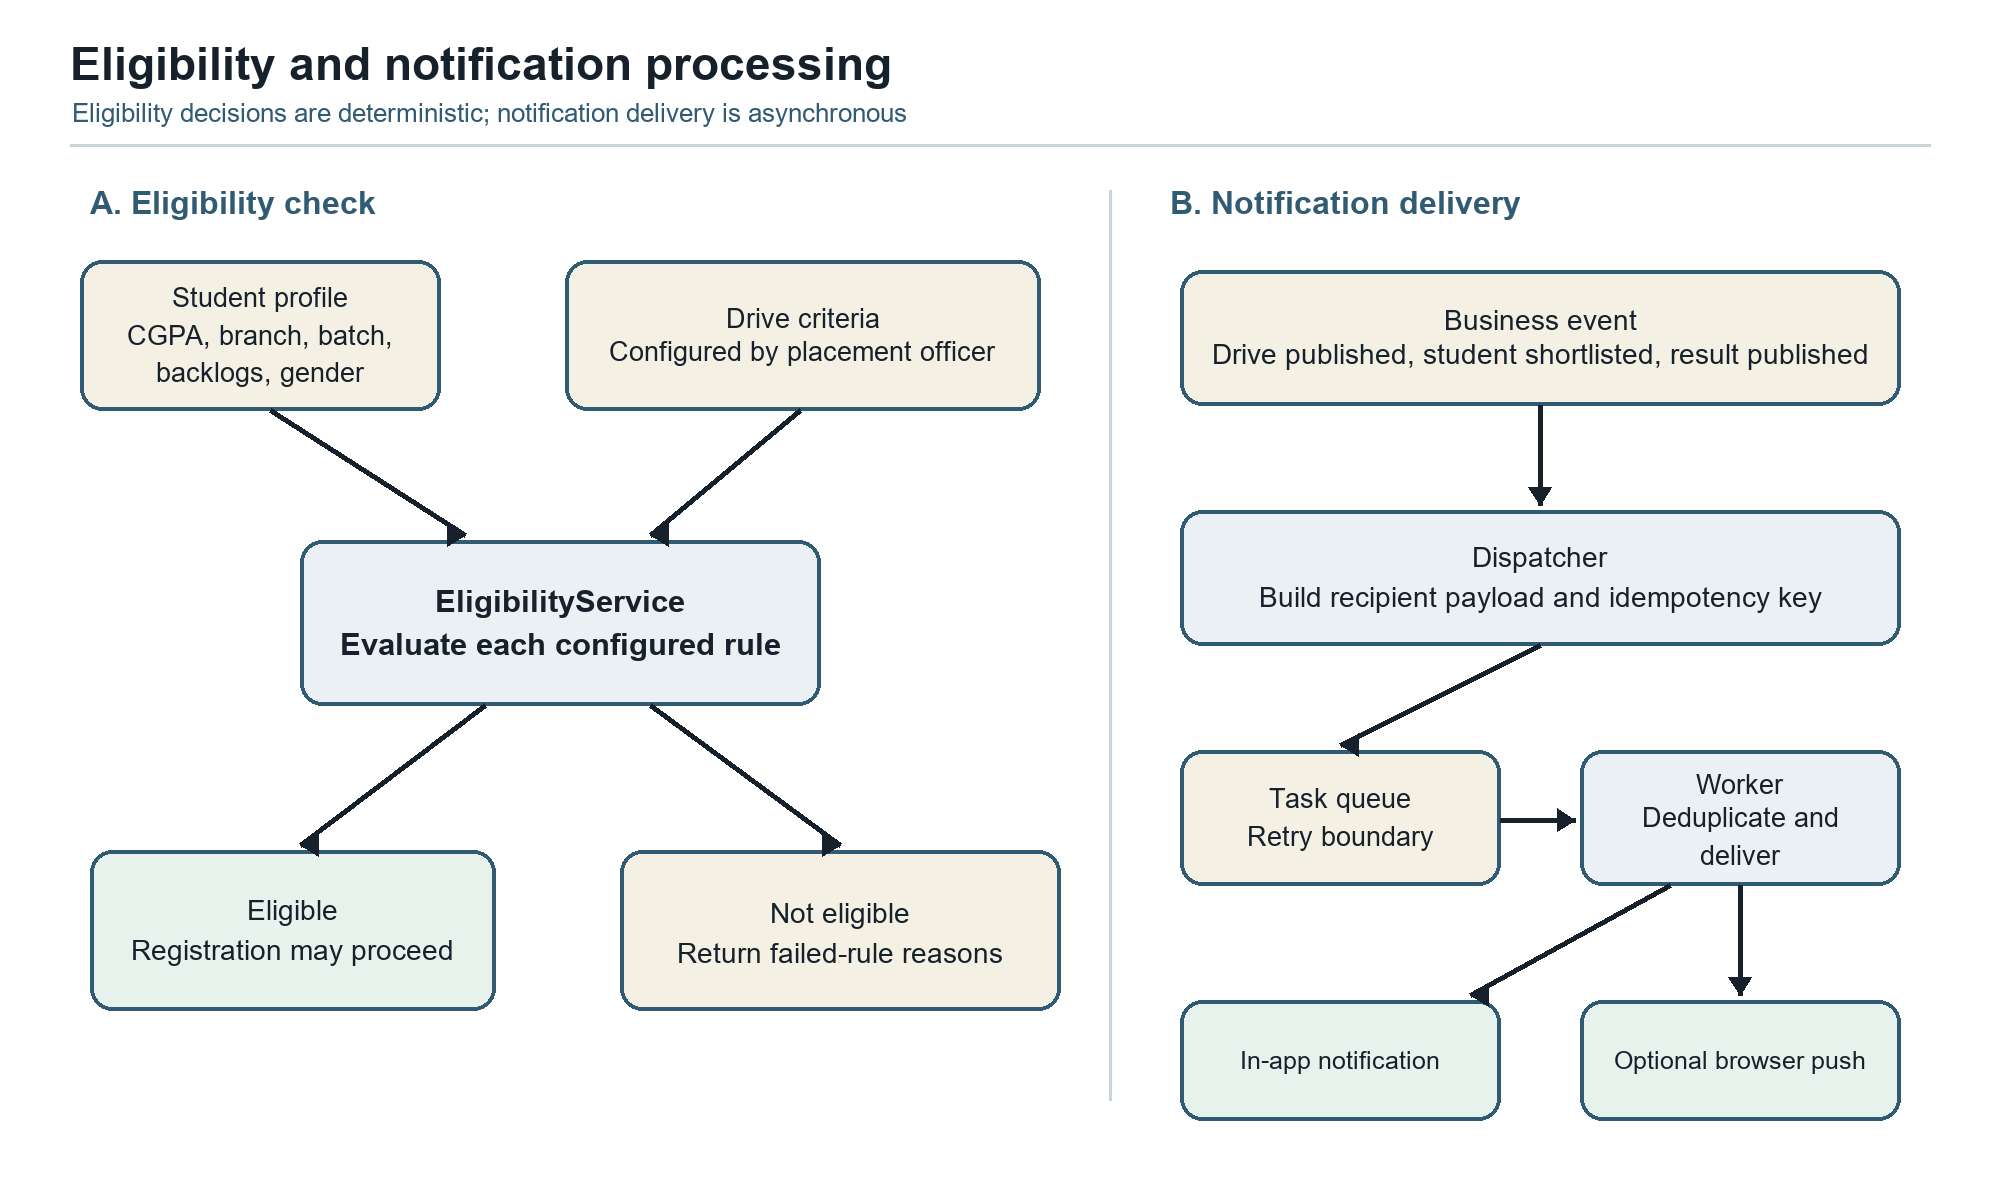
\includegraphics[width=0.86\textwidth]{eligibility_notifications.png}
\caption{Deterministic eligibility evaluation and asynchronous notification delivery.}
\label{fig:eligibility-notifications}
\end{figure*}

\subsection{Registration, Stages, and Notifications}
Registration is permitted only while a drive accepts applications and after eligibility requirements are satisfied. Registration records link a student to a drive and are used by officer views for applicant review. Officers assign shortlisted candidates to ordered stages, publish schedules and instructions, and record decisions. A student's progress is represented by application and stage records rather than inferred from a single free-text status.

Notifications are dispatched as individual recipient tasks. The dispatcher forms an idempotency key from notification type, reference identifier, and recipient identifier before enqueueing work. The worker persists an in-app notification and can deliver browser push when an active subscription is available. The per-recipient design isolates retries and avoids requiring the original HTTP request to synchronously perform all delivery. Figure~\ref{fig:eligibility-notifications} shows both processes.

Table~\ref{tab:events} summarizes representative events and their intended recipients.

\begin{table}[!t]
\caption{Placement Events and Notification Recipients}
\label{tab:events}
\centering
\footnotesize
\begin{tabular}{p{0.35\columnwidth} p{0.53\columnwidth}}
\toprule
\textbf{Event} & \textbf{Recipient rule} \\
\midrule
Drive published & Students eligible for the published drive \\
Deadline reminder & Eligible students who have not registered \\
Registration confirmed & The registering student \\
Stage shortlist & Students assigned to that stage \\
Stage schedule updated & Students assigned to the affected stage \\
Result published & Students with an outcome for the drive \\
\bottomrule
\end{tabular}
\end{table}

The design combines centralized transactional data with asynchronous work. The database remains the source of truth for profiles and drive state, while the task queue handles delivery that can be retried independently. Idempotency keys help the worker reject duplicate work, although they do not prove exactly-once delivery by an external push service.

\subsection{Security and Access Control}
CampusFlow separates capabilities by user role and applies authorization at the backend API. This follows the RBAC principle of assigning permissions to roles [2], while ownership checks restrict student-scoped resources to their owner. The security regression tests exercise forbidden student access to administrative endpoints, internal task endpoints, and another student's private resources. These checks are important because a frontend-only restriction would not prevent a caller from invoking the API directly.

Authentication uses short-lived access tokens and refresh-token handling; the project documentation specifies RS256-signed JWTs [3]. Student documents are designed for private object storage. The production security design also describes audit records for state-changing operations. Deployment claims such as live cloud key rotation, external push-provider reliability, and production penetration-test results are outside the evidence reported in this paper.

\section{Implementation}
The frontend is built with React, TypeScript, Vite, Tailwind CSS, and Zustand. It presents role-specific workflows and calls the versioned HTTP API. The backend uses FastAPI, SQLAlchemy's asynchronous data-access support, and PostgreSQL. Alembic manages schema migrations. The code separates API routing, services, repositories, ORM models, and Pydantic schemas so that HTTP validation and authorization are not mixed with database query construction.

The placement-drive service validates state transitions and writes audit records as the drive changes state. The eligibility service is a pure rule evaluation over a student profile and a criteria dictionary; it returns a boolean and a list of explanatory strings. The notification dispatcher constructs task payloads and idempotency keys, while the worker is responsible for persistence and delivery. The separation allows the API to enqueue notification work without making push delivery part of the student's or officer's request latency.

Table~\ref{tab:implementation} lists the principal technologies used by the project.

\begin{table}[!t]
\caption{Implementation Environment}
\label{tab:implementation}
\centering
\small
\begin{tabular}{p{0.34\columnwidth} p{0.54\columnwidth}}
\toprule
\textbf{Component} & \textbf{Technology} \\
\midrule
Frontend & React, TypeScript, Vite, Tailwind CSS, Zustand \\
Backend API & Python, FastAPI \\
Persistence & PostgreSQL, SQLAlchemy 2.0 \\
Schema migrations & Alembic \\
API validation & Pydantic \\
\bottomrule
\end{tabular}
\end{table}

The deployment architecture describes cloud services for document storage and asynchronous notifications. The repository's automated workflow test substitutes a local task service and invokes the worker directly. It therefore verifies application-level task handling, not Cloud Tasks dispatch latency or external browser-push delivery in a production environment.

\subsection{Request and Data Flow}
For a student eligibility request, the API authenticates the caller, loads the requested drive and the caller's profile, reads the drive's criteria, and invokes the eligibility service. The result is attached to the response and is not an ML-generated probability. On registration, the service checks the drive state and eligibility before creating a drive--student association. For shortlisting, an officer submits student identifiers for a stage; the service persists assignments and dispatches notifications to affected students. These paths preserve the same ownership and role checks regardless of the user interface.

Table~\ref{tab:api} lists representative endpoints used by these flows. The paths shown are versioned API routes; authorization is checked by the backend.

\begin{table}[!t]
\caption{Representative Placement API Operations}
\label{tab:api}
\centering
\footnotesize
\begin{tabular}{p{0.21\columnwidth} p{0.68\columnwidth}}
\toprule
\textbf{Operation} & \textbf{Purpose} \\
\midrule
Drive listing & Authenticated users view drives available to their role. \\
Eligibility check & Student's profile is evaluated against one drive's criteria. \\
Drive registration & Eligible student registers while the drive is open. \\
Stage shortlisting & Officer assigns registered students to a stage. \\
Notification retrieval & User reads their own in-app notifications. \\
\bottomrule
\end{tabular}
\end{table}

\subsection{Design Decisions}
Table~\ref{tab:decisions} explains several choices visible in the implementation and architecture documentation.

\begin{table}[!t]
\caption{Design Decisions and Their Rationale}
\label{tab:decisions}
\centering
\footnotesize
\begin{tabular}{p{0.27\columnwidth} p{0.61\columnwidth}}
\toprule
\textbf{Decision} & \textbf{Reason and consequence} \\
\midrule
Rule-based eligibility & Mirrors explicit drive criteria and supports reason messages; it does not rank or predict candidate success. \\
Forward-only drive states & Prevents accidental lifecycle rollback; corrections require an explicit administrative process. \\
Modular monolith & Keeps domain modules in one deployable application for an institution-scale product; modules can be separated later if load warrants. \\
Per-recipient notification tasks & Isolates retries and deduplication by recipient; queue configuration and external delivery still require deployment testing. \\
\bottomrule
\end{tabular}
\end{table}

\section{Experiments and Evaluation}
The repository includes integration tests using synthetic users and database records. The test setup selects a dedicated test database, recreates the schema for each test, and uses an in-process HTTP client to call the FastAPI application. No real student records are needed for the scenarios described here.

The main workflow test creates an officer and a synthetic student, creates a company-linked drive with criteria, adds a stage, publishes the drive, opens registration, checks the student's eligibility, registers the student, shortlists the student, processes notification tasks, and verifies that the student can retrieve a shortlist notification. A separate security scenario asserts that student credentials do not authorize administrator or internal scheduler/task operations. Unit tests check analytics percentage calculations and zero-denominator behavior.

Table~\ref{tab:evaluation} summarizes the scenarios represented by these test cases. It reports assertions encoded in the repository, not a claim that the tests were executed during preparation of this paper.

\begin{table}[t]
\caption{Functional Test Scenarios Represented in the Repository}
\label{tab:evaluation}
\centering
\small
\begin{tabular}{p{0.26\columnwidth} p{0.61\columnwidth}}
\toprule
\textbf{Test scenario} & \textbf{Assertions represented in the test suite} \\
\midrule
Placement lifecycle & Eligible student can view a drive, register, and be shortlisted by an officer. \\
Notification flow & Worker processing creates an in-app shortlist notification. \\
Access control & Student requests to admin and internal endpoints are rejected. \\
Analytics calculations & Zero-denominator cases return zero percentages; percentage calculations are checked with synthetic values. \\
\bottomrule
\end{tabular}
\end{table}

The test fixtures provide a repeatable way to validate business paths and access boundaries. They do not measure throughput, latency, concurrent-user capacity, notification-provider success rates, or usability. The tests also do not show whether actual placement outcomes improve. Consequently, this paper reports no MAE, accuracy, response-time, scale, or satisfaction figures.

\subsection{Evaluation Protocol for a Deployment Study}
A deployment study should test each eligibility rule, invalid transitions, duplicate registrations, notification retries, and role boundaries. Report the load-test environment, concurrency, and latency percentiles. A usability study requires institutional approval and privacy review.

\section{Discussion}
CampusFlow models placement as linked records and explicit state transitions. A drive, its criteria, a student's registration, and stage assignments remain connected, giving officers a traceable progress view and students an explanation for eligibility decisions.

The design has trade-offs. Rule-based checks cannot assess whether configured thresholds are fair or current, and incorrect academic records can produce incorrect decisions. Criteria therefore need authorized review and a correction procedure. Forward-only drive states improve consistency but require auditable handling of exceptional corrections.

Asynchronous dispatch separates requests from notification delivery, but retries cannot guarantee external push delivery. In-app records remain the persistent channel; push depends on browser permission and provider availability. Analytics summarize stored data and do not establish that CampusFlow improves placement outcomes.

Evaluation is limited to automated test scenarios with synthetic records. No load test, usability study, deployment study, or manual-process comparison is reported; operational effectiveness at university scale remains unknown.

\subsection{Limitations and Future Work}
The present system does not establish interoperability with a university identity provider, an employer applicant-tracking system, or a national student database. The reported tests also do not evaluate bulk notification throughput, backup recovery, accessibility with assistive technology, or the effect of profile corrections on every active application. Future work should conduct a deployment study with institution-approved synthetic or de-identified data, recruit students and placement staff for usability tasks, and measure API latency and queue delivery under a published workload. A future study should also assess eligibility-policy governance, privacy controls, and audit-log review with the institution's placement office.

\section{Conclusion}
This paper described CampusFlow, a university placement-management system that links student profiles, company and drive administration, deterministic eligibility, registration, recruitment stages, notifications, and analytics. The system uses a modular FastAPI backend, a React and TypeScript client, PostgreSQL persistence, role- and ownership-aware authorization, and asynchronous notification processing. Its repository contains synthetic integration scenarios for a cross-role placement workflow and selected security boundaries. These scenarios provide functional checks but do not quantify production performance or placement impact. A measured deployment and user study remain necessary before making effectiveness or scalability claims.

\begin{thebibliography}{00}
\bibitem{rathod2022}
N. T. Rathod and S. Shah, ``Design Paper on Online Training and Placement System (OTaP),'' \emph{International Journal of Communications}, vol. 16, no. 2, pp. 8--12, 2022, doi: 10.46300/9107.2022.16.2.
\bibitem{chaurasia2023}
S. Chaurasia, ``Student Internship Placement Management System using Python,'' \emph{International Journal of Research in Science \& Engineering}, pp. 30--49, 2023, doi: 10.55529/ijrise.33.30.49.
\bibitem{trimukhe2017}
S. Trimukhe, A. Todmal, K. Pote, M. Gite, and S. S. Pophale, ``Online Training and Placement System,'' \emph{International Journal of Advanced Research in Computer Science and Software Engineering}, vol. 7, no. 4, pp. 344--349, 2017, doi: 10.23956/ijarcsse/v7i3/0181.
\bibitem{bhaskaran2025}
H. Bhaskaran, ``Student Placement Management System,'' \emph{International Journal for Research in Applied Science and Engineering Technology}, vol. 13, no. 5, pp. 2319--2321, 2025, doi: 10.22214/ijraset.2025.70765.
\bibitem{sandhu2000}
R. Sandhu, D. Ferraiolo, and R. Kuhn, ``The NIST model for role-based access control: Towards a unified standard,'' in \emph{Proc. 5th ACM Workshop on Role-Based Access Control}, 2000, pp. 47--63, doi: 10.1145/344287.344301.
\bibitem{rfc7519}
M. Jones, J. Bradley, and N. Sakimura, ``JSON Web Token (JWT),'' RFC 7519, May 2015, doi: 10.17487/RFC7519.
\end{thebibliography}

\end{document}